% ============================================================
%  1-bit register - abstract board-level wiring (no power rails).
%  Just two boards now: a 2:1 MUX board (the mux-2-to-1 module) and a
%  D flip-flop board.
%      MUX picks  D (LD=1, load)  or  Q (LD=0, hold)  -> flip-flop -> Q
%  Q feeds back into the MUX's "0" input, so LD=0 keeps the value.
%  Compile:  pdflatex wiring.tex
% ============================================================
\documentclass[border=20pt]{standalone}
\usepackage{circuitikz}
\usetikzlibrary{calc}
\tikzset{brd/.style={rounded corners=3pt, fill=blue!6},
         ffb/.style={rounded corners=3pt, fill=orange!10}}

\begin{document}
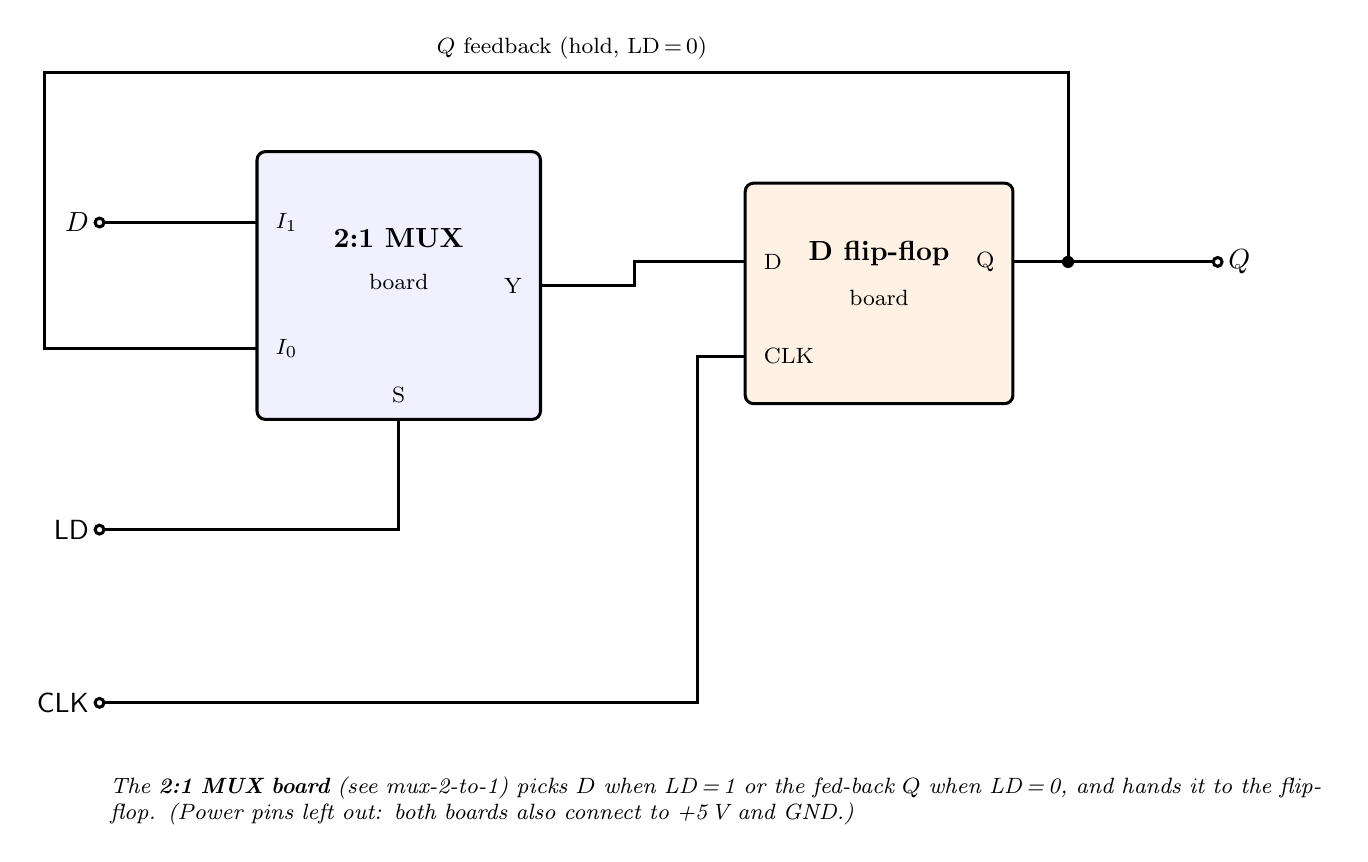
\begin{tikzpicture}[line width=1.1pt, font=\sffamily]

  % ---------- the two boards ----------
  \draw[brd] (3.0,2.2) rectangle (6.6,5.6);
  \node[font=\bfseries] at (4.8,4.5){2:1 MUX};
  \node[font=\footnotesize] at (4.8,3.95){board};
  \node[anchor=west,font=\footnotesize] at (3.1,4.7){$I_1$};
  \node[anchor=west,font=\footnotesize] at (3.1,3.1){$I_0$};
  \node[anchor=south,font=\footnotesize] at (4.8,2.28){S};
  \node[anchor=east,font=\footnotesize] at (6.5,3.9){Y};

  \draw[ffb] (9.2,2.4) rectangle (12.6,5.2);
  \node[font=\bfseries] at (10.9,4.3){D flip-flop};
  \node[font=\footnotesize] at (10.9,3.75){board};
  \node[anchor=west,font=\footnotesize] at (9.3,4.2){D};
  \node[anchor=west,font=\footnotesize] at (9.3,3.0){CLK};
  \node[anchor=east,font=\footnotesize] at (12.5,4.2){Q};

  % ---------- inputs ----------
  \draw (1.0,4.7)  node[ocirc]{} node[left]{$D$}  -- (3.0,4.7);                 % D  -> MUX I1 (the "1" input)
  \draw (1.0,0.8)  node[ocirc]{} node[left]{LD}   -- (4.8,0.8) -- (4.8,2.2);    % LD -> MUX select S
  \draw (1.0,-1.4) node[ocirc]{} node[left]{CLK}  -- (8.6,-1.4) -- (8.6,3.0) -- (9.2,3.0);

  % ---------- MUX Y -> flip-flop D ----------
  \draw (6.6,3.9) -- (7.8,3.9) -- (7.8,4.2) -- (9.2,4.2);

  % ---------- Q output + hold feedback ----------
  \draw (12.6,4.2) -- (13.3,4.2) coordinate (qt) -- (15.2,4.2) node[ocirc]{} node[right]{$Q$};
  \fill (qt) circle (2.2pt);
  % drop down on the far left (clear of the D input lead) so the feedback never crosses D
  \draw (qt) -- (13.3,6.6) -- (0.3,6.6) -- (0.3,3.1) -- (3.0,3.1);              % Q -> MUX I0 (the "0" input)
  \node[font=\footnotesize,anchor=south] at (7.0,6.64){$Q$ feedback (hold, LD\,=\,0)};

  \node[anchor=north west,font=\footnotesize\itshape,text width=15.5cm] at (1.0,-2.2)
        {The \textbf{2:1 MUX board} (see mux-2-to-1) picks $D$ when LD\,=\,1 or the fed-back $Q$ when
         LD\,=\,0, and hands it to the flip-flop. (Power pins left out: both boards also connect to
         +5\,V and GND.)};

\end{tikzpicture}
\end{document}
